\documentclass[tikz,border=3pt]{standalone}
\usetikzlibrary{arrows,intersections,decorations.pathreplacing}

\begin{document}

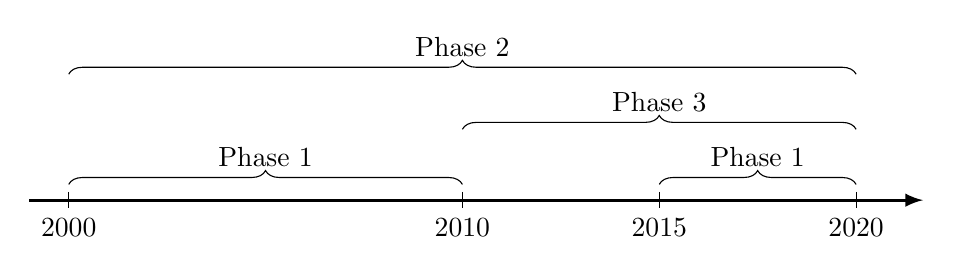
\begin{tikzpicture}
\draw[very thick,-{latex}] (0,0) -- (11.35,0) node{};
\foreach \x/\l in {0.5/2000,5.5/2010,8/2015,10.5/2020}
\draw (\x,3pt) -- (\x,-3pt) node[below]{$\l$};
\draw [decorate,decoration={brace,amplitude=5pt}]
(0.5,1.6) -- (10.5,1.6) node[midway,yshift=1em]{Phase 2};
\draw [decorate,decoration={brace,amplitude=5pt}]
(5.5,0.9) -- (10.5,0.9) node[midway,yshift=1em]{Phase 3};
\draw [decorate,decoration={brace,amplitude=5pt}]
(0.5,0.2) -- (5.5,0.2) node[midway,yshift=1em]{Phase 1};
\draw [decorate,decoration={brace,amplitude=5pt}]
(8,0.2) -- (10.5,0.2) node[midway,yshift=1em]{Phase 1};
\end{tikzpicture}

\end{document}
